\chapter{Determination of External Force Coefficient of  External Threaded Joints}
\section{Nomenclature}
	\begin{tabular}[t]{lp{7cm}}
		$ A $ & area of the raw section, $ \unit{mm^2} $\\
		$ F $ & applied force, $ \unit{N} $\\
		$ F_H $ & horizontal component of $ F $, $ \unit{N} $\\
		$ F_V $ & vertical component of $ F $, $ \unit{N} $\\
		$ J_{x'x'} $ & moment of inertia along XX-axis, $ \unit{kg\cdot mm^2} $\\
		$ k $ & safety factor\\
		$ V $ & tightening force, $ \unit{N} $\\
		$ V_{max} $ & maximum tightening force, $ \unit{N} $\\
		
	\end{tabular}
\begin{tabular}[t]{lp{7cm}}
	$ W $ & bending moment of the raw section, $ \unit{N\cdot mm} $\\
	$ y_{max} $ & maximum distance, $ \unit{mm} $\\
	$ z $ & a coefficient\\
	$ \alpha $ & contact angle, $ \unit{^\circ} $\\
	$ \chi $ & external force coefficient\\
	$ \bar{\chi} $ & average value of $ \chi $\\
	$ \Delta F $ & force difference between each experiment, $ \unit{N} $
\end{tabular}

\section{Aim}
\begin{enumerate}
	\item Help students understand clearly about the method of determination of the
	external force coefficient by theory.
	\item Help students calculate the tightening force in the case of force acting in any
	direction.
	\item Help students approach to the methods, instruments and determine the tightening
	force, deal with the experimental results to determine the external force
	coefficient.
\end{enumerate}

\section{Technical rules on safety}
Students must comply with the technical rules on safety in the laboratory.

\section{Experimental report}
Each group conducts the experiment with the given $ \alpha $ and $ F $\\
$ \alpha = -5^\circ $\\
$ F = 303.6\unit{(N)} $\\
$ \Delta F = 15\unit{(N)} $
\begin{figure}
	\centering
	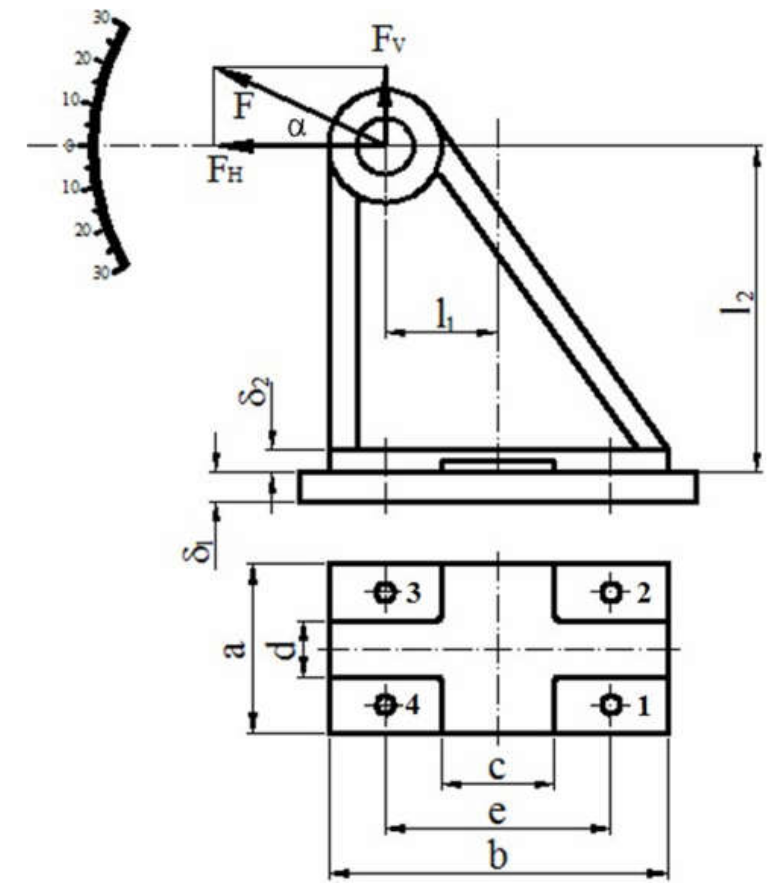
\includegraphics[width=150mm]{modelexp4.png}
	\caption{Model of experimental calculation}
	\label{exp4fig}
\end{figure}
\subsection{Theoretical calculation of the external force coefficient}
Measuring the size of bolts and assembled details to determine the external force
coefficient by using theory.
\subsection{Calculating $ V $}
\begin{equation}
	V = \dfrac{k}{z}\left(F_V+\dfrac{MA}{W}\right) = \dfrac{k}{z}\left(F_V+\dfrac{MA_{yc}}{J}\right)(1-\chi)
	\label{safety3}
\end{equation}
\begin{equation}
	V = \dfrac{kF_H+(1-\chi)fF_V}{f_z}
	\label{tight_force}
\end{equation}
According to formulas (\ref{safety3}) and (\ref{tight_force}), selecting V max for these two values.\\
Note: The tightening force for surfaces not separated is defined by the formula:
\[V = \dfrac{k}{z}\left(\dfrac{(F_Vl_1\pm F_Hl_2)Ay_{max}}{J_{x'x'}}-F_V\right)(1-\chi)\]
\begin{tabular}{ll}
	where & $ J_{x'x'} = \dfrac{(a-b)(b^3-c^3)}{12} $\\
	& $ A = (a-d)(b-c) $\\
	& $ y_{max} = \dfrac{b}{2} $\\
\end{tabular}\vskip2mm
Tightening the bolt with the tightening force $ V = V_{max} $ (using equations \ref{safety3} and \ref{tight_force}) and
checking by measuring device.
\subsection{Measured results and process}
We increase the load by hydraulic cylinder 5 to reach values: $ F_1 $, $ F_2 $, ..., $ F_N $. They occur on the display screen (these values are less than $ F $) and fill in column 2 of Table \ref{dataexp4}. The values $ F_i = F - i\Delta F $.\\
Write down the value of tightening moment, tightening force $ V_{tni} $ by load cell method
and put them into columns 3, 4 of Tables \ref{dataexp4}.
\subsection{Calculate the external force}
Calculate the following values:
\begin{enumerate}
	\item $ F_{Vi} = F_i\sin\alpha $
	\item $ F_{Hi} = F_i\cos\alpha $
	\item $ M_i = F_{Hi}l_1\pm F_{Vi}l_2 $
\end{enumerate}
and put these values into column 5, 6 of table \ref{dataexp4}.\\
In this experiment, $ l_2 = 0 $ and $ Y_i = \dfrac{e}{2} $, therefore $ M_i = F_{Hi}l_1 $
\[V_{tni} = V_0 + \chi\left( \dfrac{F_{Vi}}{z} + \dfrac{M_1Y_1}{\sum z_iY_i^2}\right) = V_0 + \chi\left(\dfrac{F_{Vi}}{z} + \dfrac{F_{Hi}l_1\pm F_{Vi}l_2}{2e}\right)\]
where $ i=1,2,...,N $\\
Here, $ \chi $ is determined by the formula:
\[\chi_i = \dfrac{V_{tni}-V_{tn1}}{\dfrac{F_{Vi}-F_{V1}}{z} + \dfrac{(F_{Hi}-F_{H1})l_1+(F_{Vi}- F_{H1})l_2}{2e}}\]
According to the experimental model, $ z=4 $, $ e=200\unit{(mm)} $, $ l_1= 300\unit{(mm)}$, $ l_2 = 100\unit{(mm)} $ and then write down the results into column 7 of table \ref{dataexp4}.\\
Therefore, the average value of external force coefficient through $ N $ measuring times $ 18305.42 \unitp{Pa\cdot s} $
\begin{equation}
	\bar{\chi} = \dfrac{\chi_1+\chi_2+...+\chi_{N-1}}{N-1}
\end{equation}
\begin{table}[h!t]
	\centering
	\rowcolors{3}{}{lightgray!20}
	\renewcommand{\arraystretch}{1.5}
	\begin{tabular}[ht]{crrrrr}
		\toprule
		\multirow{2}{*}{No.} & \md{$ F_i $} & \md{$ V_{tni} $} & \md{$ F_{Vi} $} & \md{$ F_{Hi} $} & \md{$ \chi_i $} \\
		& \md{$ \unit{(N)} $} & \md{$ \unit{(N)} $} &\md{ $ \unit{(N)} $} & \md{$ \unit{(N)} $} & \\
		\midrule
		\rule[-1ex]{0pt}{2.5ex} 1 & 303.2 & 3025 & -26.43 & 302.05 & 0 \\
		\rule[-1ex]{0pt}{2.5ex} 2 & 287.8 & 3097 & -25.08 & 286.71 & 0.12 \\
		\rule[-1ex]{0pt}{2.5ex} 3 & 271.4 & 3221 & -23.65 & 270.37 & 0.23 \\
		\rule[-1ex]{0pt}{2.5ex} 4 & 257.8 & 3304 & -22.47 & 256.82 & 0.16 \\
		\rule[-1ex]{0pt}{2.5ex} 5 & 242.8 & 3426 & -21.16 & 241.88 & 0.25 \\
		\rule[-1ex]{0pt}{2.5ex} 6 & 227.8 & 3525 & -19.85 & 226.93 & 0.22 \\
		\bottomrule
	\end{tabular}
	\caption{The experimental results}
	\label{dataexp4}
\end{table}\vskip2mm
From the experimental results, plot the curve illustrated the relationship between $ \chi_i $ and $ F_i $.
\begin{figure}
	\centering
	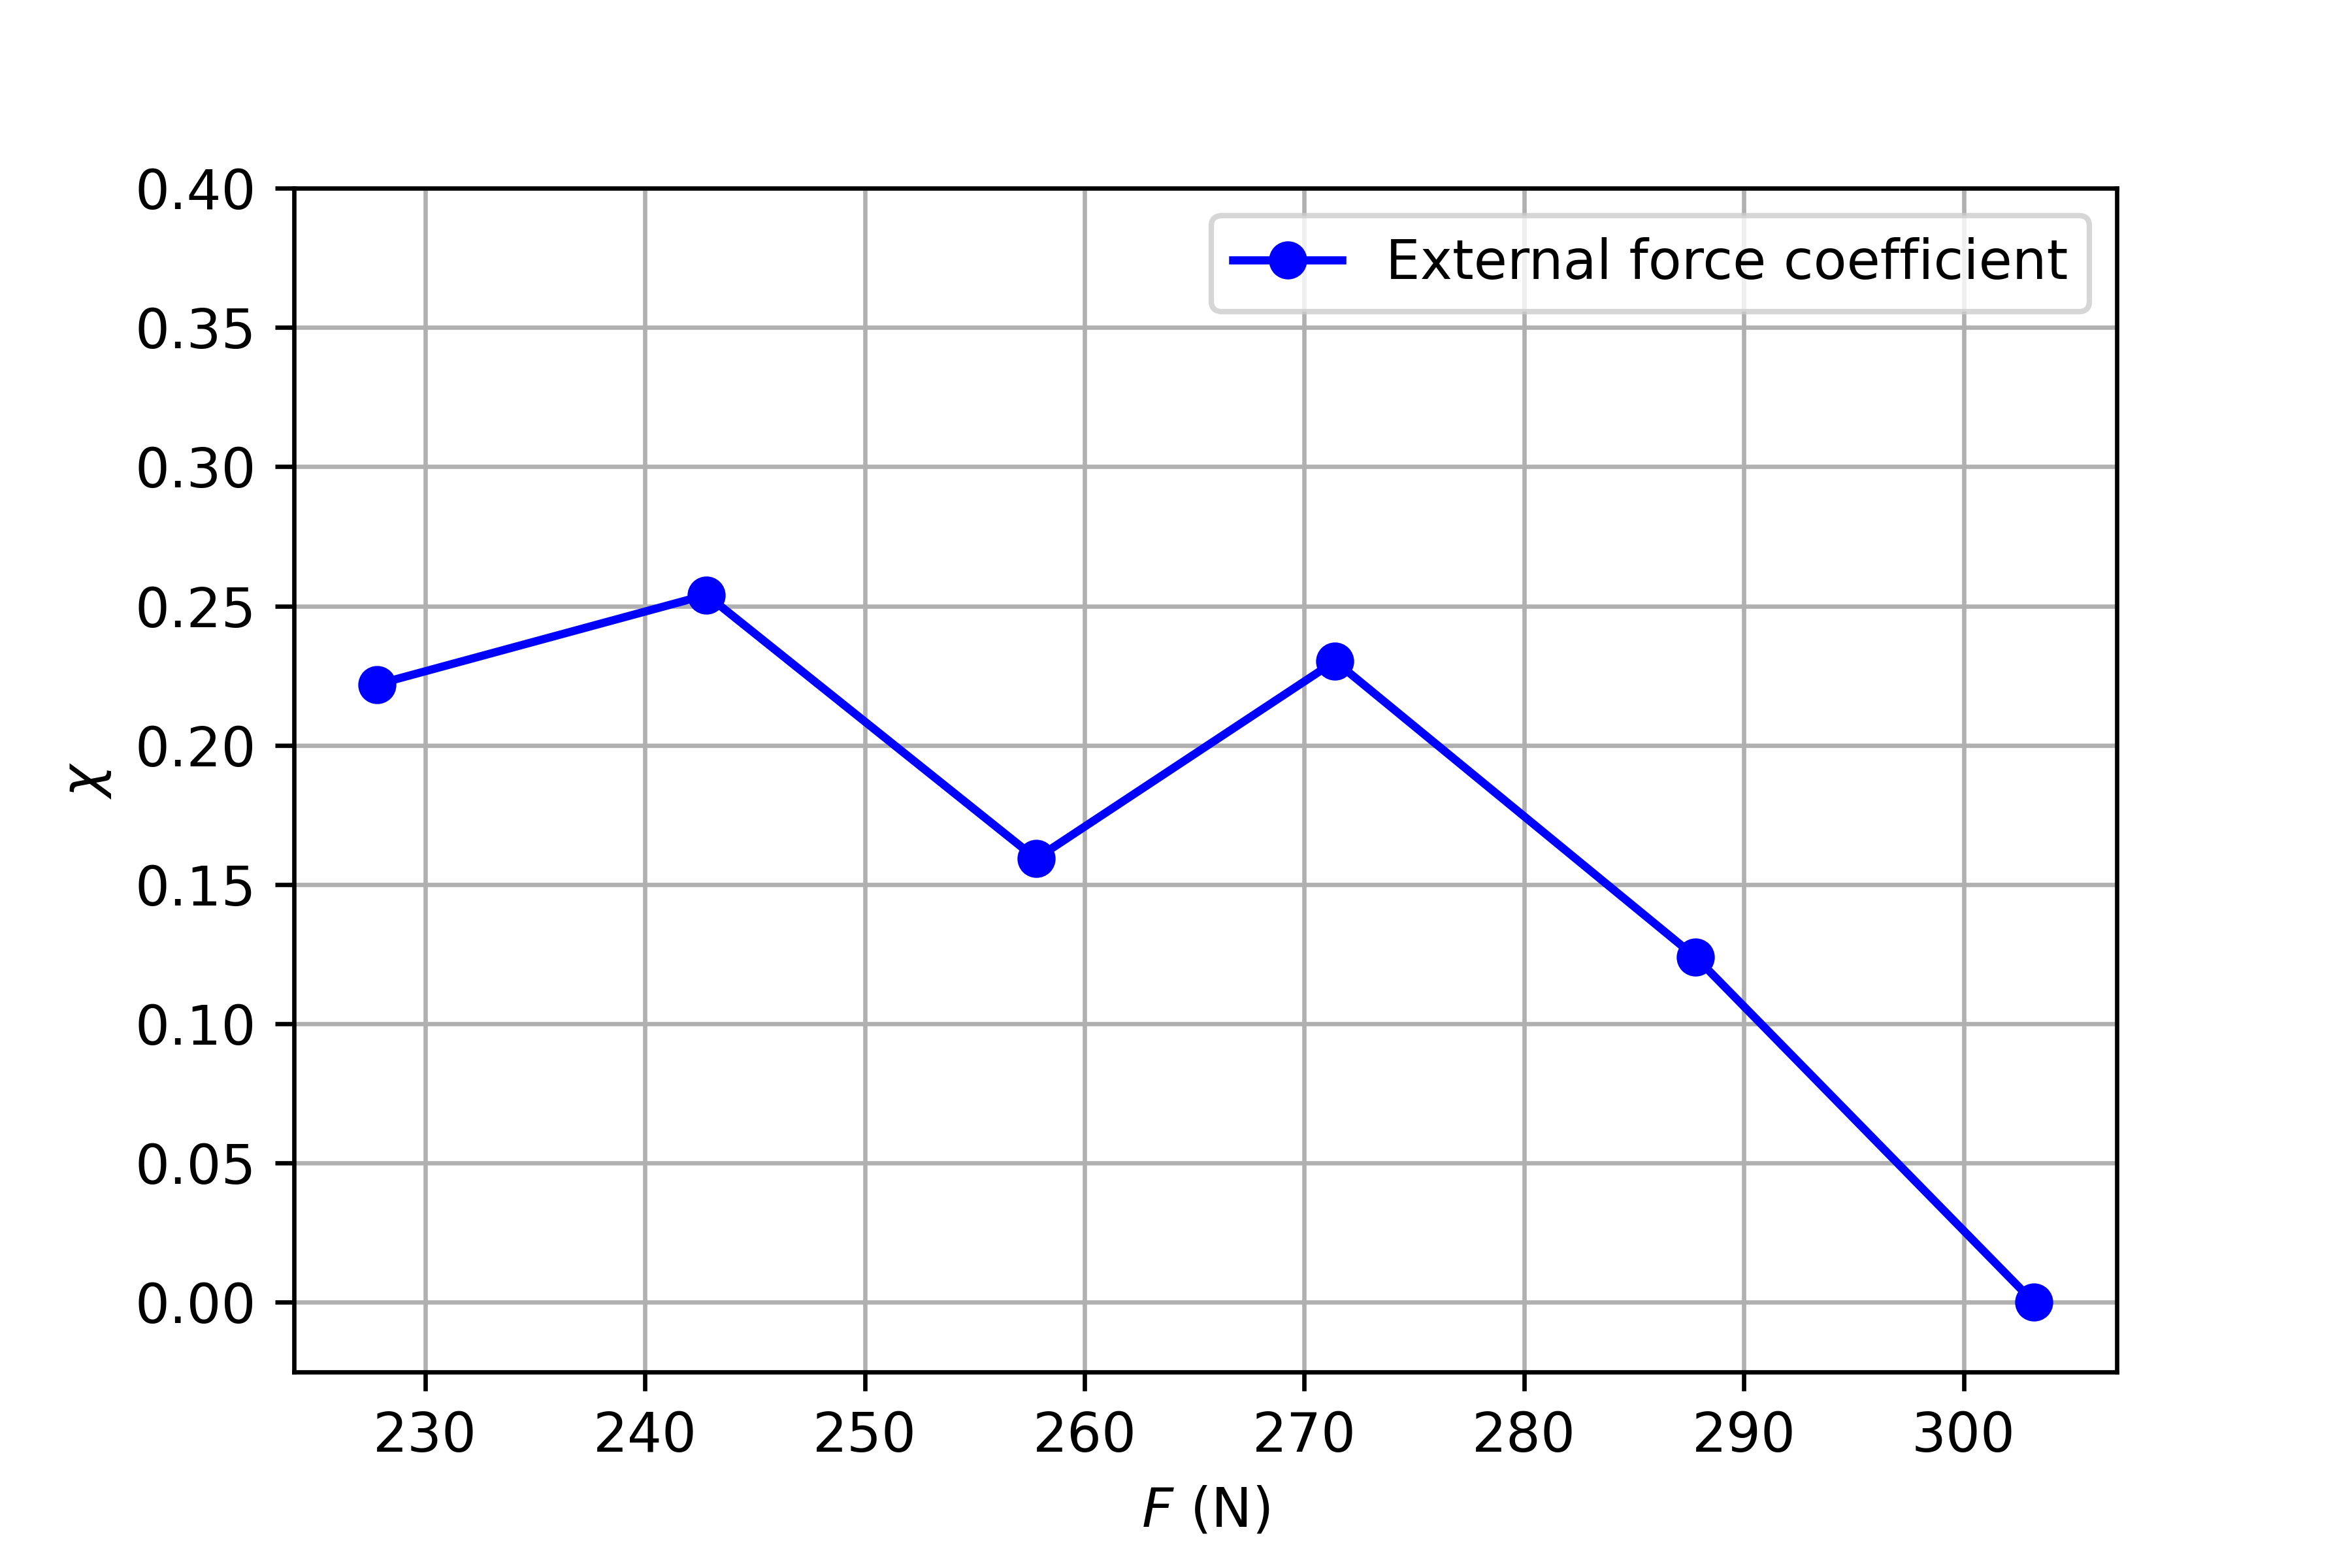
\includegraphics[width=150mm]{exp4.png}
	\caption{Relation between $ F $ and $ \chi $}
	\label{label}
\end{figure}
\section{Discussion and conclusions}
Comparing the theoretical results with experimental results and then drawing conclusions.
Possible causes of error:
\begin{itemize}
	\item Worn condition of the bolt affects the friction coefficient and thread angle.
	\item Error of the lab instrument (instability in displaying results), thus the measured values are only relative.
	\item  Rounding errors through calculations.
\end{itemize}

\section{Review questions}
\begin{enumerate}
	\item \emph{The role and importance of determining the tightening force and the tightening	moment in reality.}\\
	As mentioned, an under torqued bolt will deform and be unable to provide as much clamping force as needed. An over torqued bolt will break.
	\item \emph{The meaning of $ \chi $ and determining this coefficient by the fundamental theory.}\\
	When the joint is subjected to the external force in the non-sealed surface limitation of assemble plates, the bolt is elongated about $ \Delta l $ in length, the compression deformation of the assemble plates also reduces the same length. This means that only a part of external force $ F(\chi) $ acting on a bolt causes the extension. The other part of external force $ (1-\chi)F $ causes the decrease of the compression deformation of the assemble plates. $ \chi $ is called the external force coefficient . Therefore:
	\[\Delta l = \chi F \lambda_b = (1-\chi)F\lambda_m\]
	Where $ \lambda_b, \lambda_m $ are the flexibility of bolt and assembled parts, respectively. As a result:
	\[\chi = \dfrac{\lambda_m}{\lambda_b+\lambda_m}\]
	\item \emph{Determining the required tightening force of the bolt to avoid segregation and slip.}\\
	For assembled machine element avoid segregation and no slip, the bolt needs to be tightened with the tightening force $ V $:
	\[V = \dfrac{k}{z}\left(F_V+\dfrac{MA}{W}\right) = \dfrac{k}{z}\left(F_V+\dfrac{MA_{yc}}{J}\right)(1-\chi)\]
	\item \emph{Comparing the tightening coefficient in the cases of the joint with and without lubrication, and then drawing conclusions.}\\
	With lubrication, the tightening coefficient will decrease and vice versa. Therefore, it can be concluded that the amount of lubrication and the tightening coefficient has an inverse relationship.
\end{enumerate}